\documentclass[10pt,spanish,a4paper,openany,notitlepage]{article}
%-------------------------------------Paquetes-----------------------------------------------------------------------
\usepackage[spanish,es-tabla]{babel}  	% Traduce los textos a castellano
\usepackage[utf8]{inputenc}	% Permite escribir directamente áéíóúñ
\usepackage{t1enc}            	% Agrega caracteres extendidos al font
\usepackage{amsmath} 		%Permite imprimir mas opcciones matematicas
\usepackage{graphicx}		%Permite agregar imagenes al informe
\usepackage{multicol}  		%Permite dividir el texto en varias columnas
\usepackage{float} 		%Permite utilizar H para colocar las imagenes en un lugar especifico 
\usepackage{units}
\usepackage{circuitikz}
\usepackage{caption}
\usepackage{subcaption}
\usepackage{sidecap}
\usepackage{mathtools}
\usepackage{amssymb}
\usepackage{multirow} % Paquete para dividir las tablas en subtablas
\usepackage{booktabs} %estos 2 sirven para achicar la tabla
\usepackage{tabulary}
\usepackage{fancyhdr} % encabezado
\usepackage{textcomp} % para usar ° con el comando \textdegree
\usepackage{anysize}		%Permite modificar los margenes del documento
\usepackage{abstract} % paquete para el resumen del articulo
 
%---------------------------------------Configuraciones de pagina----------------------------------------------
\marginsize{2.5cm}{2.5cm}{1cm}{1cm}

\pagestyle{fancy}
\fancyhf{}
\lhead{
66.25 - \textsc{Dispositivos Semiconductores}\\ 
2\textsuperscript{do} Cuatrimestre de 2014
}
\rhead{
\includegraphics[width=3cm]{imagenes/FIUBA_ALTA.jpg}}
\rfoot{Página \thepage}

%---------------------------------------Definiciones propias---------------------------------------------------------
\newcommand{\oiint}{\displaystyle\bigcirc\!\!\!\!\!\!\!\!\int\!\!\!\!\!\int} %Integral doble cerrada

\DeclarePairedDelimiter\abs{\lvert}{\rvert}%
\DeclarePairedDelimiter\norm{\lVert}{\rVert}%
% Swap the definition of \abs* and \norm*, so that \abs
% and \norm resizes the size of the brackets, and the 
% starred version does not.
\makeatletter
\let\oldabs\abs
\def\abs{\@ifstar{\oldabs}{\oldabs*}}
%
\let\oldnorm\norm
\def\norm{\@ifstar{\oldnorm}{\oldnorm*}}
\makeatother
%--------------------------------------------------------------------------------------------------------------------------------


\makeatletter
\let\ps@plain\ps@fancy 
\makeatother

% lo siguiente es para borrar el titulo del resumen y que no ocupe espacio:
 \AtBeginDocument{%
 \renewcommand{\abstractname}{}%
 }
\renewcommand{\absnamepos}{empty} % originally center
 

\begin{document}
\title{\textbf{TP N\textdegree3: Dispositivos de potencia}}
\author{
  Accifonte, Franco - 93799\\
  \texttt{franco.accifonte@gmail.com}  
  \and
  Iturria, Germán  - 86270 \\
  \texttt{german.iturria@gmail.com}
  \and
   Vázquez, Matías - 91523\\
  \texttt{mfvazquez@gmail.com}
}
\date{20 de noviembre de 2014}
\maketitle

\begin{abstract} %Resumen
\emph{En este trabajo se analizará el funcionamiento de dos dispositivos 
semiconductores de potencia: el IGBT y el tiristor. En el caso del IGBT 
se modificará tanto el circuito de gate como el circuito de carga con 
el fin de analizar su comportamiento bajo diversas situaciones.
Luego se analizará el comportamiento de un tiristor bajo distintas 
condiciones circuitales y de disparo.}
\end{abstract}

\section{Parte I: IGBT}

\subsection{Análisis preliminar}

Se analizó cualitativamente el funcionamiento del circuito de la figura
\ref{fig:igbt}.

\begin{figure}[H]
\centering
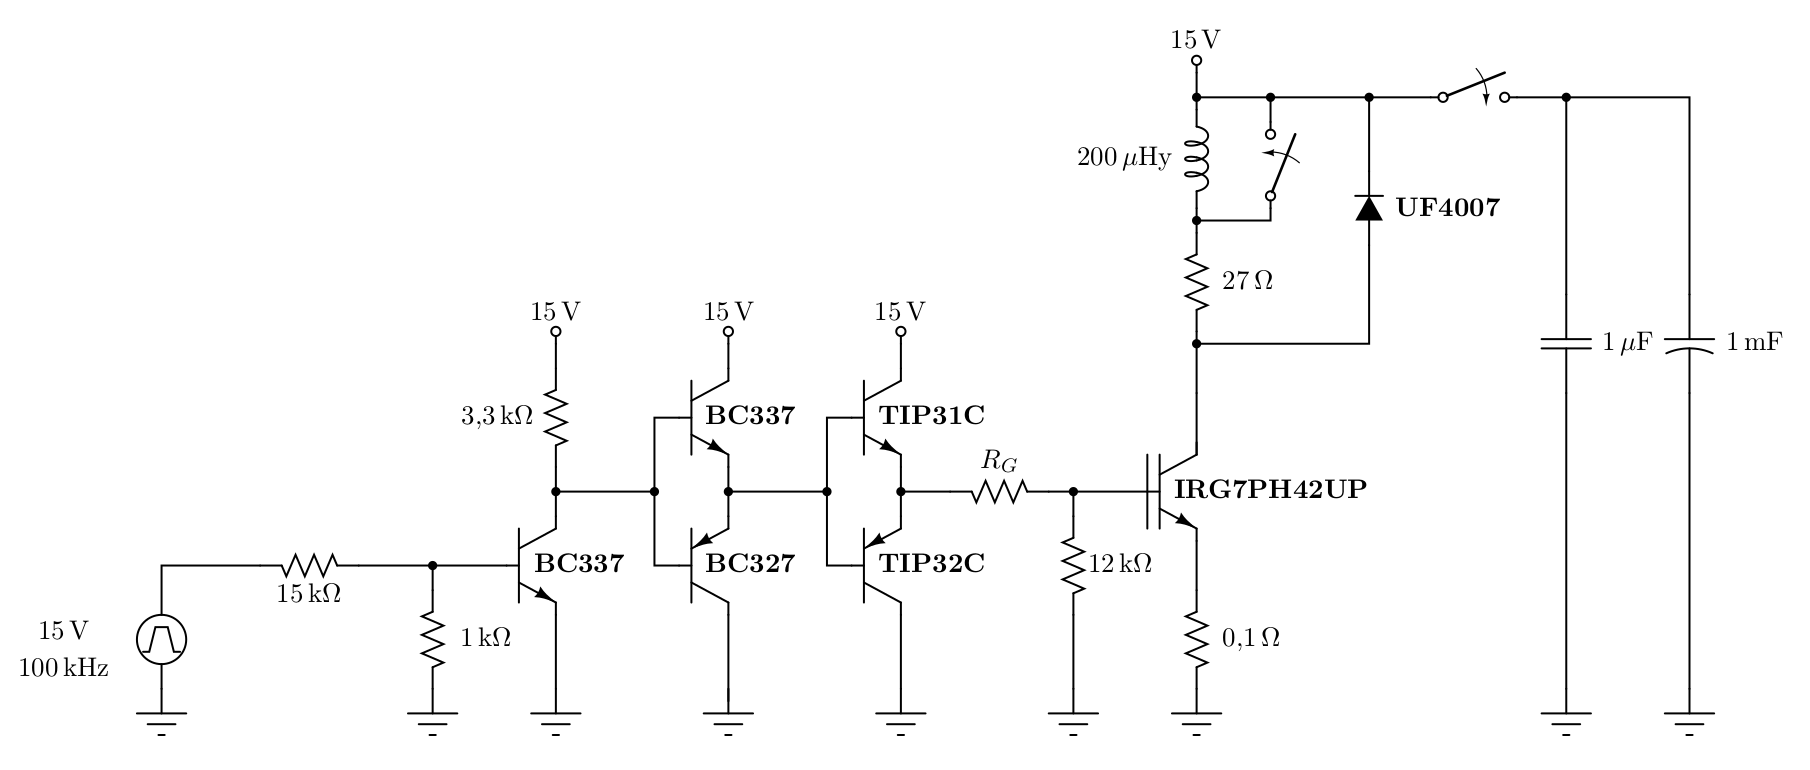
\includegraphics[scale=0.23]{./imagenes/igbt.png}
\caption{Circuito simplificado de disparo de un IGBT.}
\label{fig:igbt}
\end{figure}

\begin{itemize}
\item{Explicar por qué los transistores ocupan el lugar que ocupan, es decir, 
por que es necesario que cada etapa tenga la capacidad de manejar cada 
vez más corriente.}

Se necesita que la corriente que entrega la etapa final sea alta. Para 
lograr esto se conectan varias etapas consecutivas de transistores y, 
dado que cada etapa amplifica la corriente que recibe de la etapa anterior, 
es necesario que cada etapa sea capaz de manejar corrientes superiores 
a la etapa anterior.

\item{Identificar qué función cumple $R_G$ en el circuito. 
¿Qué sucede si $R_G=18\,\unit{\Omega}$ o $R_G=1\, \unit{k\Omega}$?}

La función que cumple $R_G$ en el circuito es cargar o descargar más 
rápido el capacitor asociado al IGBT. Mientras más chica sea $R_G$, 
menor será el tiempo necesario para que el transistor conmute su estado.

\item{¿Qué función cumple el diodo {\bf UF4007}?}

Cuando el inductor no está cortocircuitado y el transistor pasa de 
saturación a corte, el inductor generará una corriente para mantener el 
flujo magnético. Si el diodo no está conectado, el único camino que tiene 
esta corriente para circular es a través del transistor, y puede llegar 
a dañarlo. Al conectarse el diodo, se facilita un camino por donde circular 
esta corriente inductiva sin dañar el transistor.

\end{itemize}

\subsection{Mediciones del circuito}

Con la ayuda de una placa experimental, donde se encuentra implementado
el circuito, se realizaron las siguientes mediciones utilizando un
osciloscopio digital del que se obtuvieron los datos numéricos.
Con la ayuda del programa de cálculo numérico \emph{Octave} se obtuvieron
gráficos de las mediciones realizadas.

\subsubsection{Caída de tensión y corriente sobre $R_G$}

\begin{figure}[H]
\centering
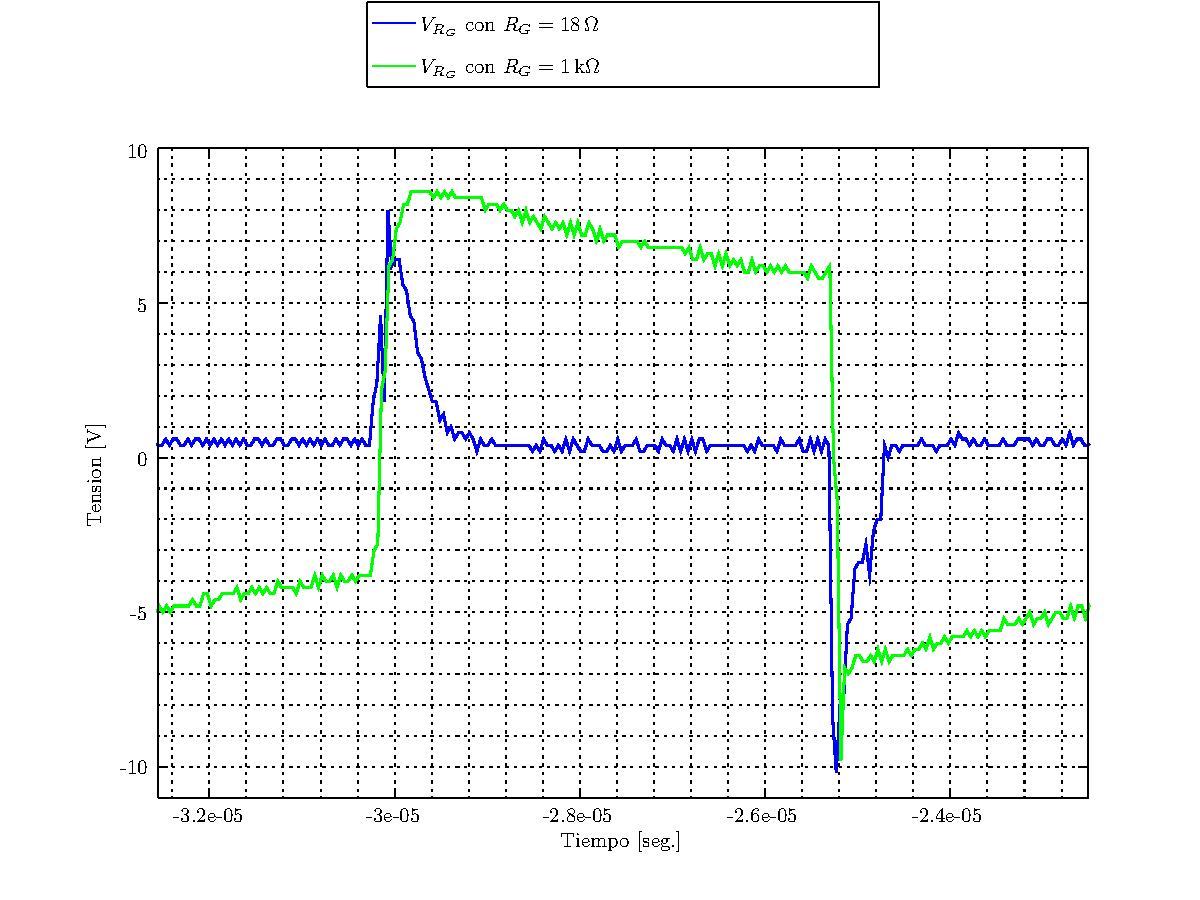
\includegraphics[scale=0.65]{./Octave/IGBT/Vr.pdf}
\caption{Caída de tensión en $R_G$.}
\label{fig:V_RG}
\end{figure}

Para estimar la corriente máxima registrada con cada resistencia, 
simplemente se buscó el valor máximo de tensión sobre $R_G$ y se 
obtuvo la corriente planteando la ley de Ohm.

\begin{itemize}

\item Para $R_G=18\,\unit{\Omega}$:

\[ \displaystyle I_{G,max}=444\,\unit{mA} \]

\item Para $R_G=1\,\unit{k\Omega}$:

\[ \displaystyle I_{G,max}=8.8\,\unit{mA} \]

\end{itemize}

Como se puede observar en el gráfico de la figura \ref{fig:V_RG} para
$R_G = 18\, \unit{\Omega}$ el capacitor asociado al IGBT logra cargarse
antes de que termine el pulso, ya que la corriente es mayor, por lo tanto
el IGBT logra conmutar su estado.

Para $R_G = 1\, \unit{k\Omega}$ durante el pulso la tensión no llega
a cero ya que el capacitor no logra cargarse durante el pulso y por lo tanto el IGBT no
logra conmutar su estado.\\

Las siguientes mediciones se realizaron con $R_G = 18\, \unit{\Omega}$
ya que con dicho valor logra conmutar su estado.

\subsubsection{Capacidad de entrada}

A partir de la variaciòn en la tensión de \emph{Gate} y la corriente de
carga del IGBT, se obtuvo la capacidad de entrada mediante la ecuación
\ref{eq:capacidad}.

\begin{equation}
I_G = C_{IGBT} \frac{\partial V_G}{\partial t}
\label{eq:capacidad}
\end{equation}

Se obtuvo el rango de valores $4.44\, \unit{nF} \leqslant C_{IGBT} \leqslant 6.67\, \unit{nF}$.
cuando el capacitor asociado al IGBT se encuentra cargado.

\subsubsection{Corriente de salida y potencia con el inductor cortocircuitado}

\begin{figure}[H]
\centering
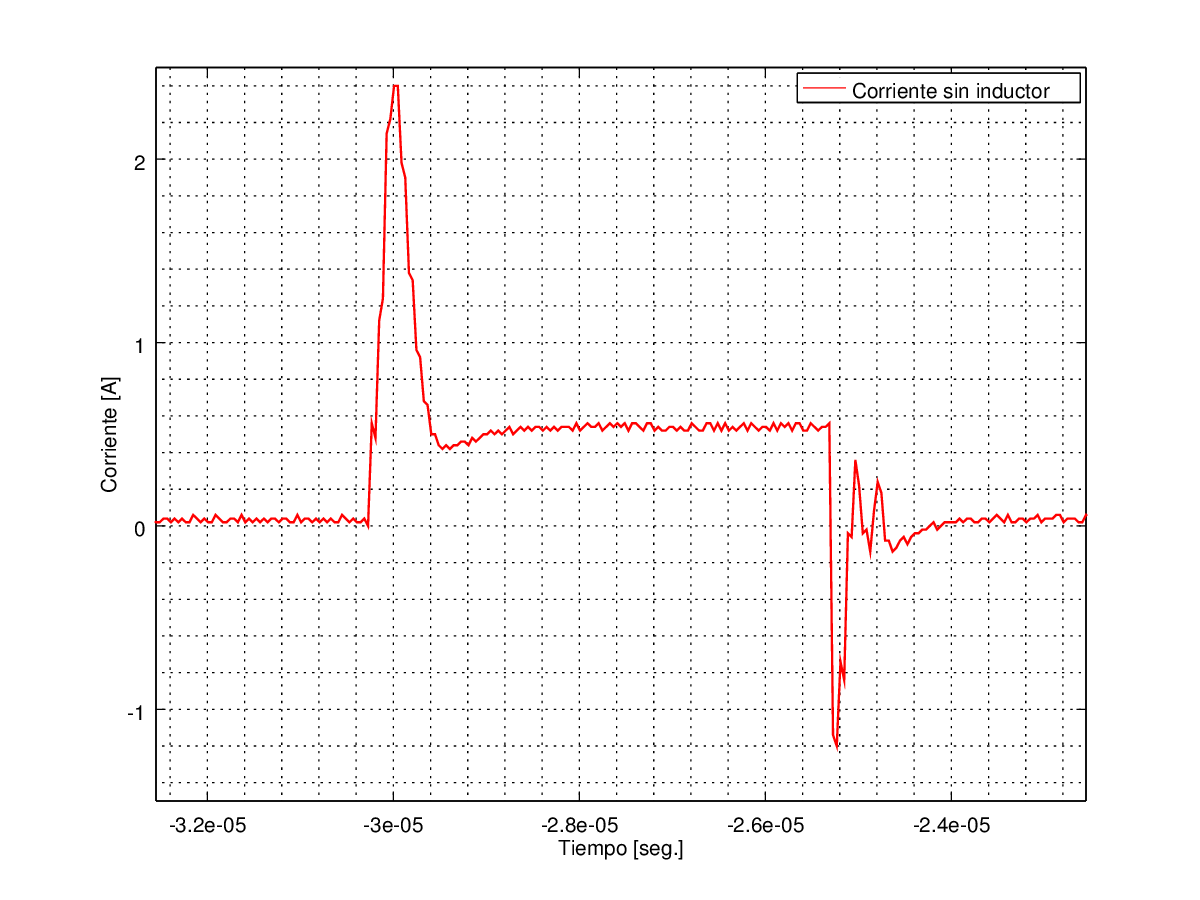
\includegraphics[scale=0.65]{./Octave/IGBT/corriente_sin_L.png}
\caption{Corriente de salida con el inductor cortocircuitado.}
\label{fig:corriente_sin_L}
\end{figure}

En el gráfico de la figura \ref{fig:P_sin_L} se puede observar la potencia 
instantánea. Calculada mediante la ecuación \ref{eq:P_instantanea}.

\begin{equation}
P(t) = I_{E}\, V_{CE}
\label{eq:P_instantanea}
\end{equation}

\begin{figure}[H]
\centering
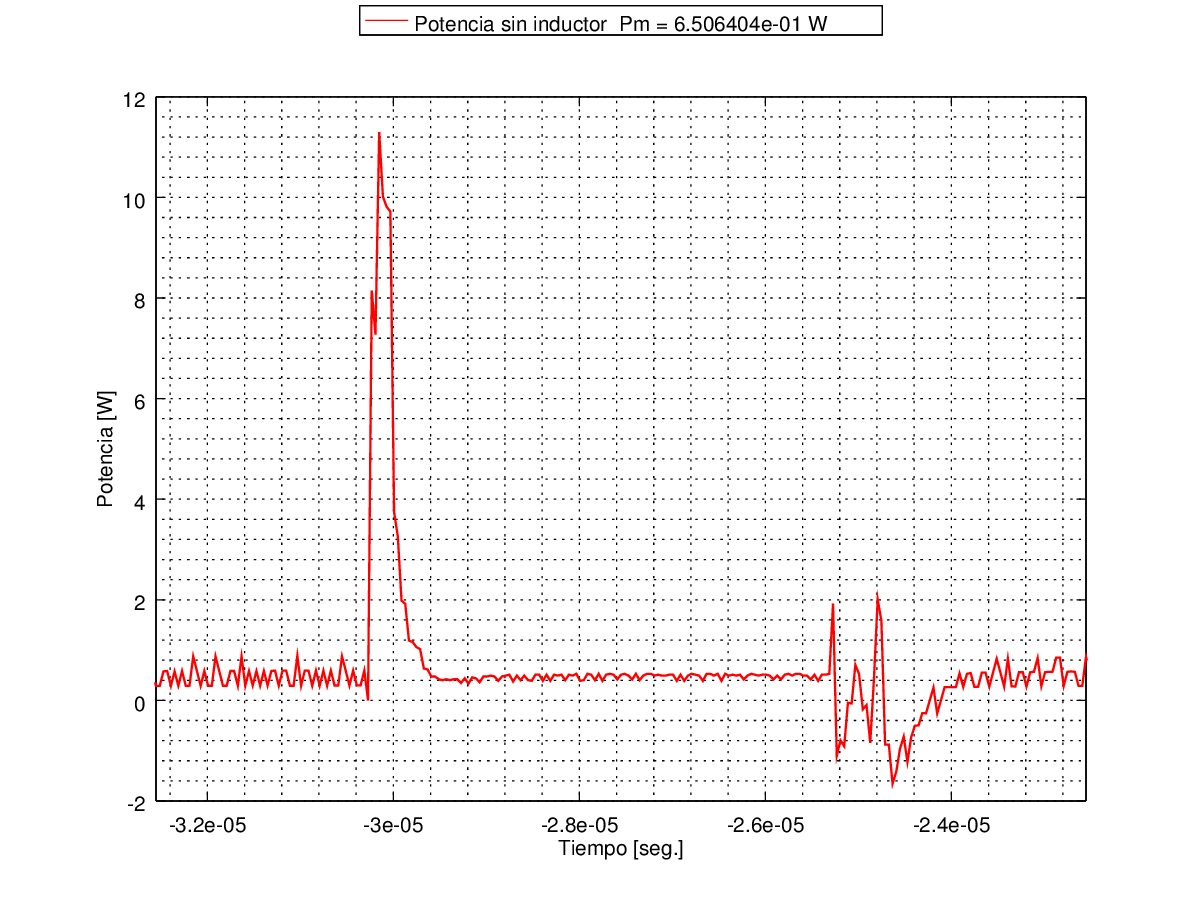
\includegraphics[scale=0.65]{./Octave/IGBT/Potencia_sin_L.png}
\caption{Potencia instantánea con el inductor cortocircuitado.}
\label{fig:P_sin_L}
\end{figure}

La potencia media se obtuvo mediante la ecuación \ref{eq:P_m}\footnote{Se 
utilizó la regla del trapecio para aproximar la integral.}.


\begin{equation}
P_m = \frac{1}{T}\, \int_0^T \! P(t) \, dt
\label{eq:P_m}
\end{equation}

Se obtuvo:

\[ \displaystyle P_m=650.6\,\unit{mW} \]

Luego se calculó la potencia eficaz mediante la ecuación \ref{eq:P_eficaz}

\begin{equation}
P_{ef} = \sqrt{\frac{1}{T}\, \int_0^T \! P^2(t) \, dt}
\label{eq:P_eficaz}
\end{equation}

Se obtuvo:

\[ \displaystyle P_{ef}= 1.6134\,\unit{W} \]

\subsubsection{Corriente de salida y potencia sin cortocircuitar el inductor}

Se repitió la medición anterior sin cortocircuitar el inductor. Se obtuvieron
los siguientes resultados.

\begin{figure}[H]
\centering
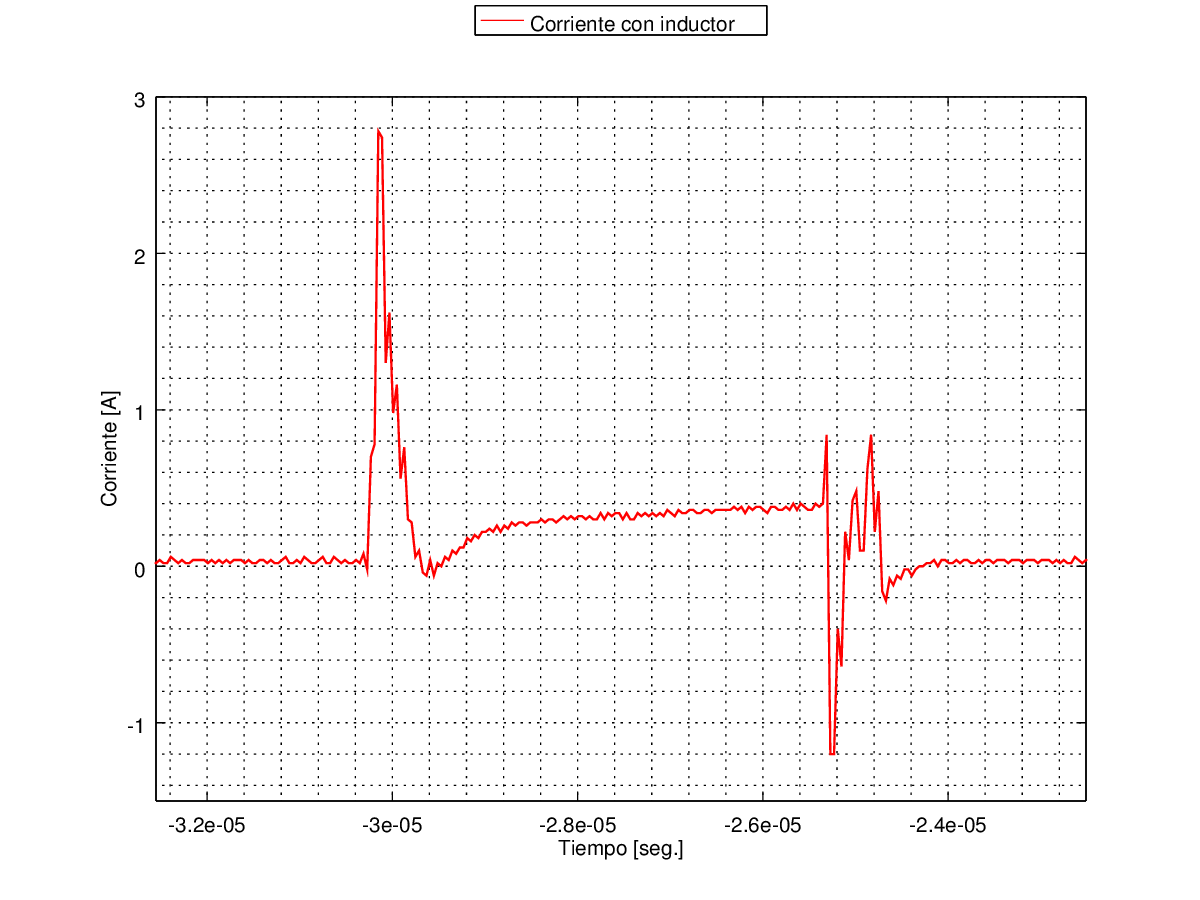
\includegraphics[scale=0.65]{./Octave/IGBT/corriente_con_L.png}
\caption{Corriente de salida sin cortocircuitar el inductor.}
\label{fig:corriente_con_L}
\end{figure}

\begin{figure}[H]
\centering
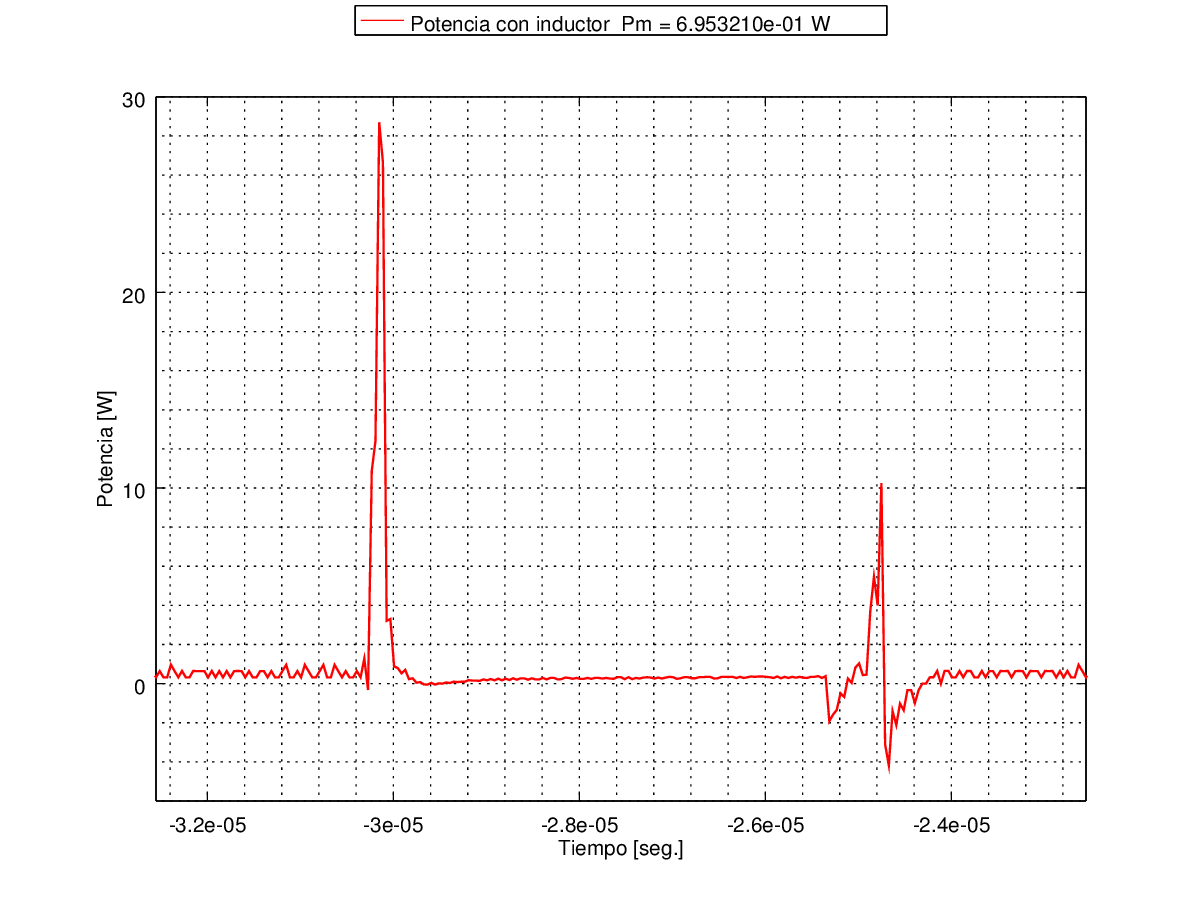
\includegraphics[scale=0.65]{./Octave/IGBT/Potencia_con_L.png}
\caption{Potencia instantánea sin cortocircuitar el inductor.}
\label{fig:P_m}
\end{figure}

\[ \displaystyle P_m=695.3\,\unit{mW} \]

\[ \displaystyle P_{ef}= 2.8865\,\unit{W} \]

\subsection{Análisis de resultados}

\begin{itemize}
\item ¿Porque es necesario entregar mucha corriente al \emph{Gate} del IGBT?
¿Qué importancia tiene la resistencia serie del circuito que se encarga de 
controlar el \emph{Gate} de este dispositivo?

La capacidad asociada al IGBT tiene un valor elevado, entonces para llegar 
a la tensión de umbral es necesario entregarle mucha carga, en otras 
palabras mucha corriente.
La importancia de la resistencia serie del circuito controlador del 
\emph{Gate} es que regula la corriente que llega al \emph{Gate}. 
Mientras mayor sea el valor de $R_G$ mayor será el 
tiempo requerido para la conmutación del transistor. Entonces sería 
deseable un valor de $R_G$ pequeño para que el IGBT llegue a conmutar 
su estado.


\item ¿Qué ocurre si se desea controlar el IGBT con una salida digital 
típica de un microcontrolador, donde la máxima corriente que puede 
entregar es de algunos pocos $\unit{mA}$?

Esta situación sería comparable a tener un valor de $R_G$ elevado. 
La corriente que llega al gate del transistor es pequeña, por lo tanto 
el tiempo que se requiere para acumular carga suficiente para conmutar 
su estado es mayor. Puede incluso ocurrir que el transistor no llegue a 
conmutar su estado dentro del período de la señal, como ocurrió cuando 
se usó $R_G=1\,k\unit{\Omega}$.

\item A partir de la estimación de potencia disipada y de los datos 
térmicos de las hojas de datos, realizar el análisis térmico del IGBT y 
calcular la temperatura de juntura.

Aplicando el modelo térmico equivalente visto de la figura 
\ref{circuito:modelo_termico} se pueden obtener las temperaturas deseadas. 

Se extrajeron de la hoja de datos los siguientes valores, considerando
la temperatura ambiente $T_a=25ºC$.
 
\begin{itemize}
\item $R_{jc}=0.39\,\unit{^oC/W}$
\item $R_{ca}= R_{cj} - R_{aj} = -R_{jc} + R_{ja} = -0.39 + 40 = 39.61\,\unit{^oC/W}$
\end{itemize}
 
Luego se planteó el modelo térmico equivalente:
 
\begin{figure}[H]
\centering
\begin{circuitikz}[american]\shorthandoff{>}
\draw
(6,0)  node[ground]{}
to [V, l=$T_a$, ] (3,0)
to [short] (0,0)
to [I, l_= $P$, v^>=$T_j - T_a$] (0,3)
to [R, l_=$R_{jc}$] (3,3)
to [R, l_=$R_{ca}$, v^=$T_c - T_a$] (3,0)
;\end{circuitikz}
\caption{Modelo térmico equivalente del IGBT}
\label{circuito:modelo_termico}
\end{figure}
 
Y se plantearon las ecuaciones del circuito para obtener la temperatura
de la juntura $T_j$

\[ \displaystyle T_c-T_a=R_{ca}\,P \]

Entonces:

\begin{equation}
T_c=R_{ca}\,P+T_a
\label{eq:T_c}
\end{equation}

Luego:

\[ \displaystyle T_j-T_c=R_{jc}\,P \]

Reemplazando la ecuación \ref{eq:T_c} se obtiene:

\begin{equation}
T_j=R_{jc}\,P+R_{ca}\,P+T_a
\label{eq:T_j}
\end{equation}

Con la ecuación \ref{eq:T_j} calculamos $T_j$ cortocircuitando el inductor y
sin cortocircuitar.

\begin{itemize}
\item Con inductor cortocircuitado. $P_m = 650.6 \, \unit{mW}$

\[ \displaystyle T_j =  51.024\, \unit{^o C}\]

\item Sin cortocircuitar el inductor. $P_m = 695.3 \, \unit{mW}$

\[ \displaystyle T_j = 52.812\, \unit{^o C} \]
\end{itemize}




\item ¿Por qué varía la corriente del IGBT con y sin el inductor conectado?

El inductor impide los saltos de corriente debido a que genera un campo 
magnético que se opone a la corriente. Por esta razón al conmutar el 
IGBT la corriente comienza desde los $0\, \unit{mA}$ y aumenta su valor 
sin sobresaltos hasta llegar a la corriente que se obtiene sin el 
inductor cuyo valor es aproximadamente $I_C \approx 0.6\, \unit{mA}$.

\end{itemize}

\section{Parte II: Tiristores}

\subsection{Análisis preliminar}

Se analizó cualitativamente el funcionamiento del circuito de la figura
\ref{fig:tiristores}.

\begin{figure}[H]
\centering
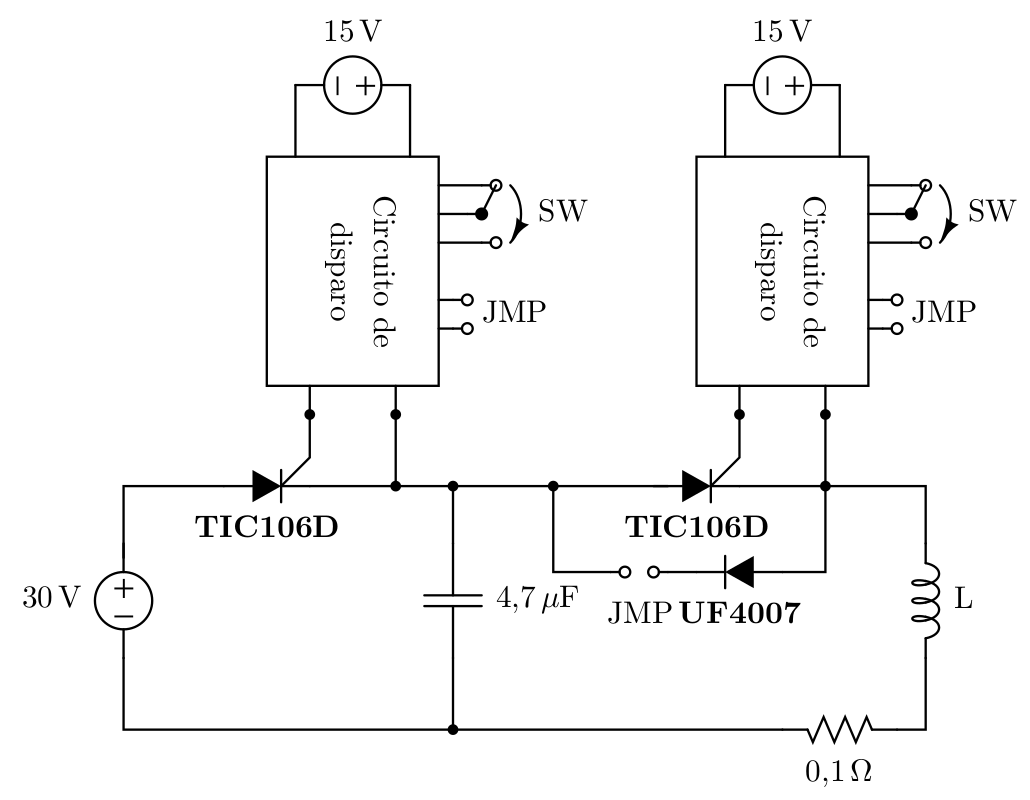
\includegraphics[scale=0.3]{./imagenes/tiristores.png}
\caption{Circuito esquemático simplificado de disparo de los Tiristores.}
\label{fig:tiristores}
\end{figure}

Se usa el primer tiristor (a la izquierda en el esquema) para cargar el 
capacitor de $4.7\,\unit{\mu F}$, y el segundo para disparar la conducción 
de un circuito RLC por lo que se espera ver la respuesta transitoria de 
dicho circuito.
Sin embargo, cuando no está conectado el diodo, la respuesta del circuito 
RLC se verá limitada por la presencia del tiristor, que impedirá que 
la corriente cambie de sentido. En cambio cuando el diodo está conectado, 
se podrá apreciar el transitorio del RLC en su totalidad.

\subsection{Mediciones del circuito}

\subsubsection{Disparo corto con el diodo desconectado}

\begin{figure}[H]
\centering
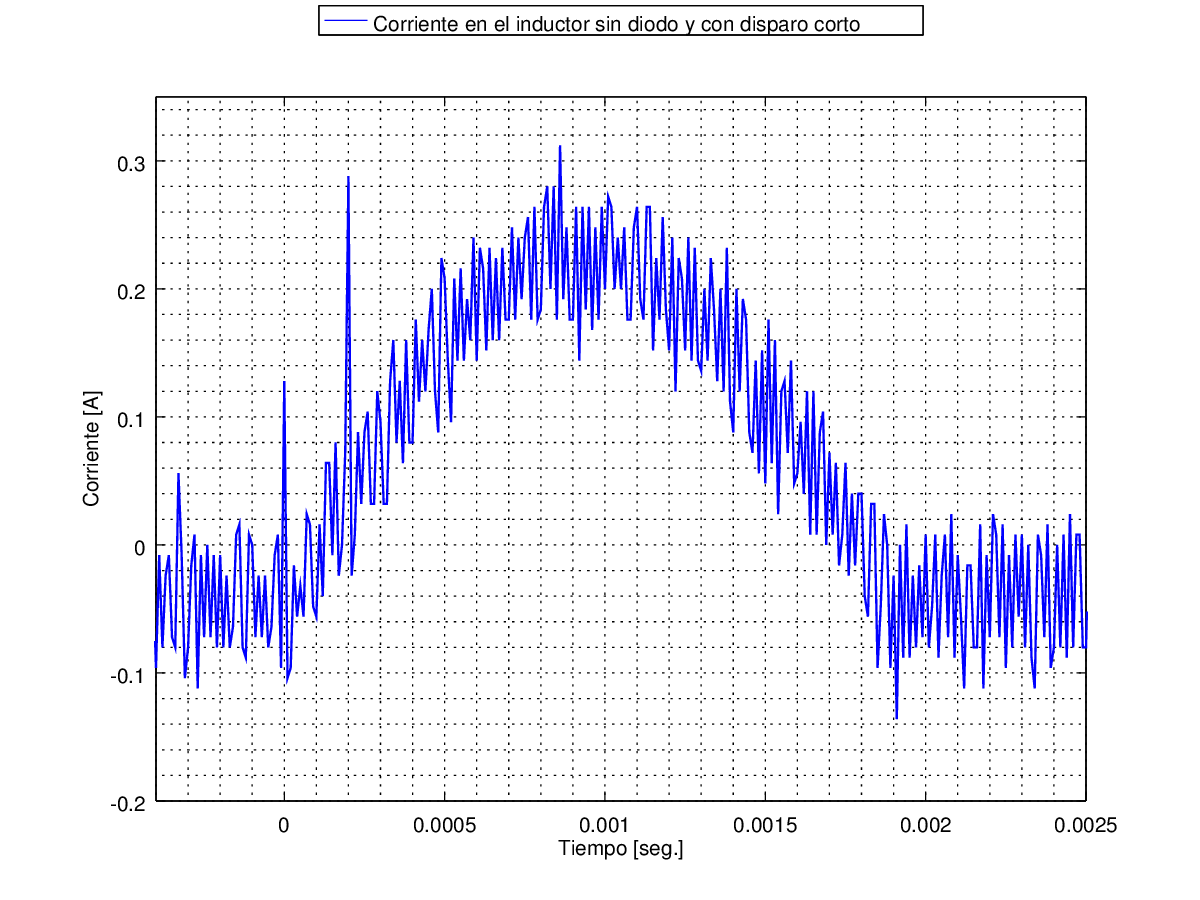
\includegraphics[scale=0.65]{./Octave/tiristores/V_L_sin_diodo_disparo_corto.png}
\caption{Tensión en el inductor respecto del terminal negativo de la fuente.}
\label{fig:V_sin_diodo_corto}
\end{figure}

\begin{figure}[H]
\centering
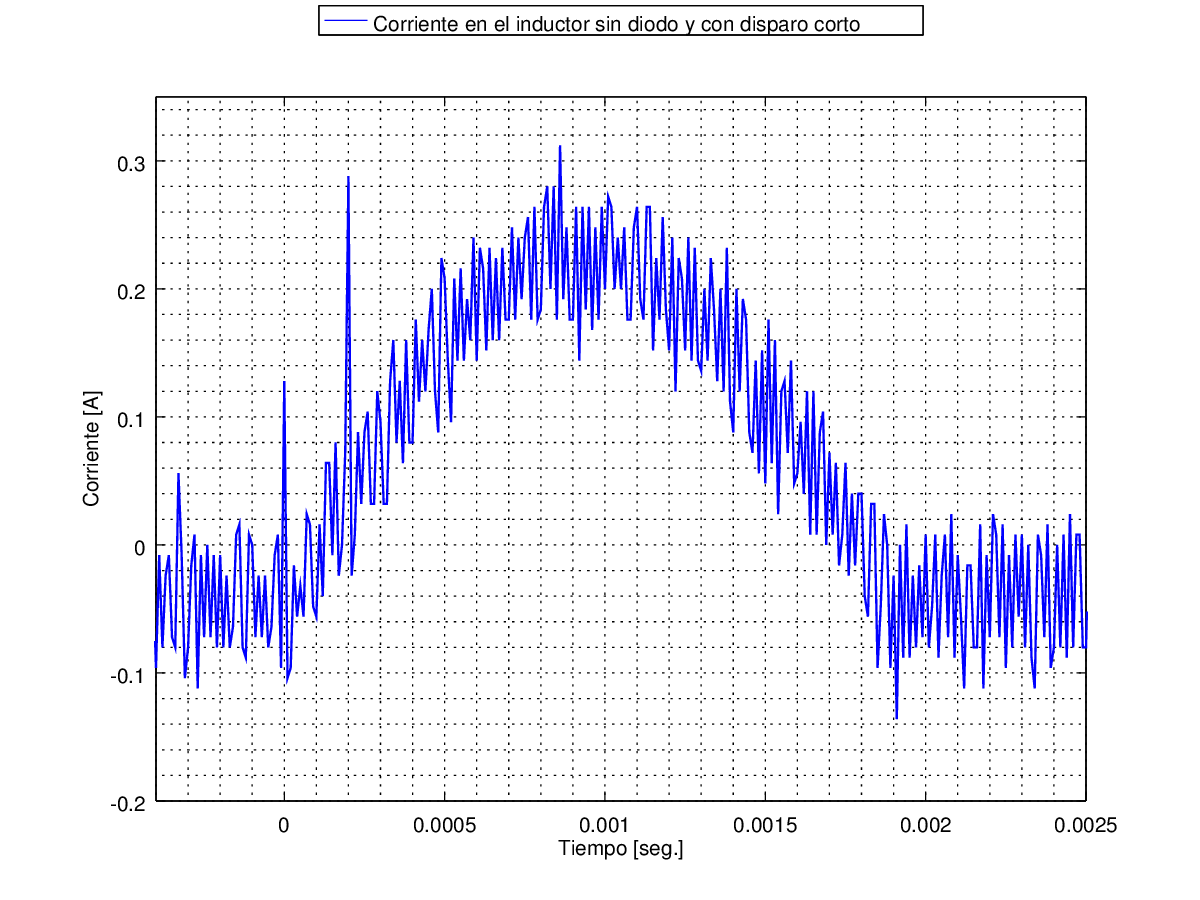
\includegraphics[scale=0.65]{./Octave/tiristores/I_L_sin_diodo_disparo_corto.png}
\caption{Corriente en el inductor respecto del terminal negativo de la fuente.}
\label{fig:I_sin_diodo_corto}
\end{figure}

\subsubsection{Disparo corto con el diodo conectado}

\begin{figure}[H]
\centering
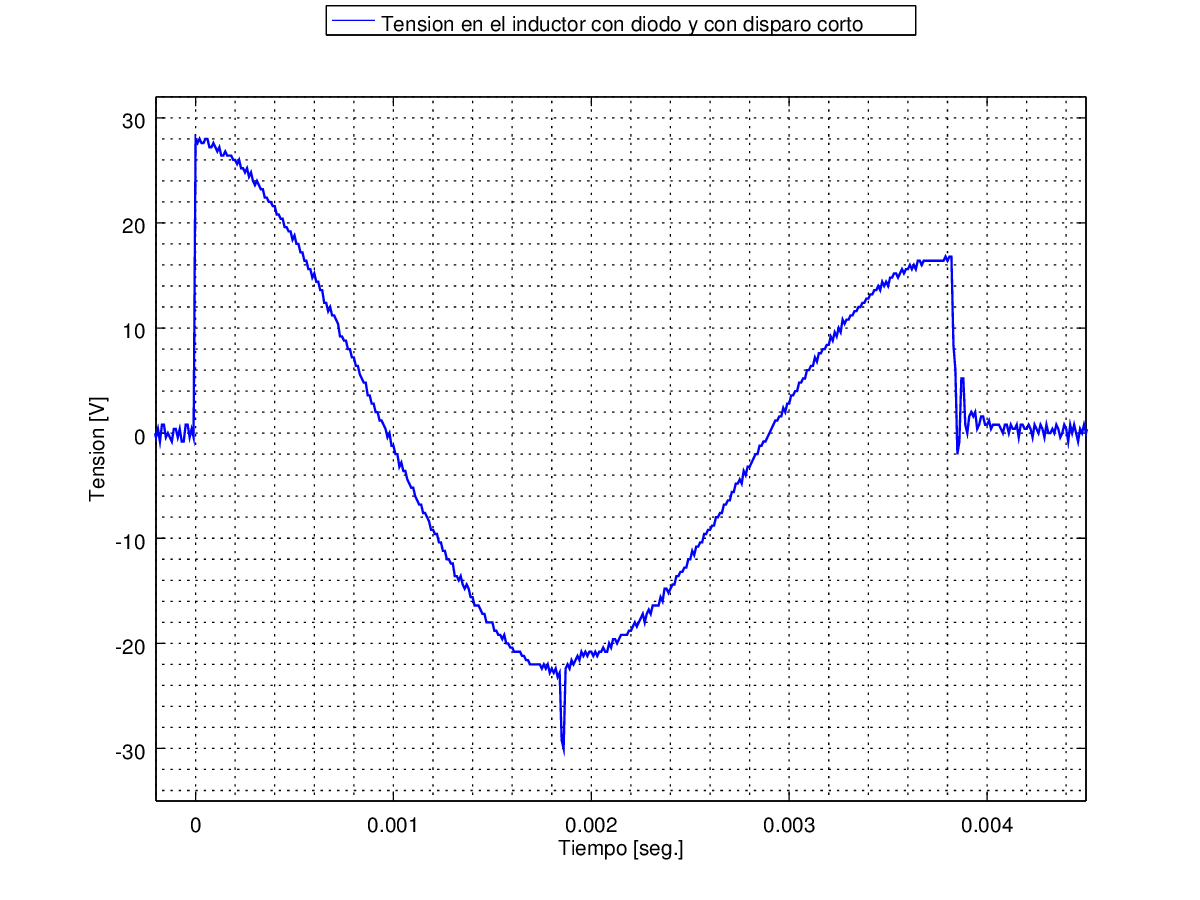
\includegraphics[scale=0.65]{./Octave/tiristores/V_L_con_diodo_disparo_corto.png}
\caption{Tensión en el inductor respecto del terminal negativo de la fuente.}
\label{fig:V_con_diodo_corto}
\end{figure}

\begin{figure}[H]
\centering
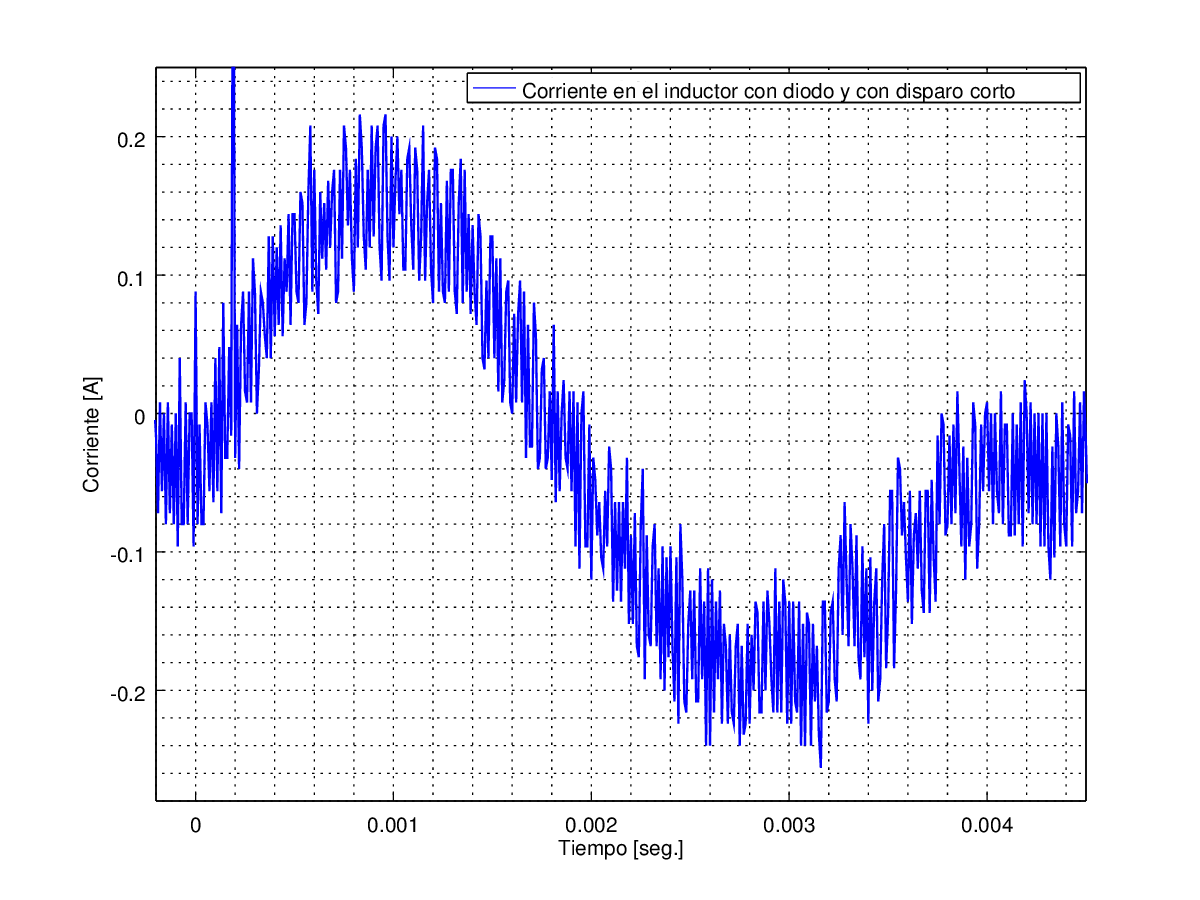
\includegraphics[scale=0.65]{./Octave/tiristores/I_L_con_diodo_disparo_corto.png}
\caption{Corriente en el inductor respecto del terminal negativo de la fuente.}
\label{fig:I_con_diodo_corto}
\end{figure}

\subsubsection{Disparo largo con el diodo conectado}

\begin{figure}[H]
\centering
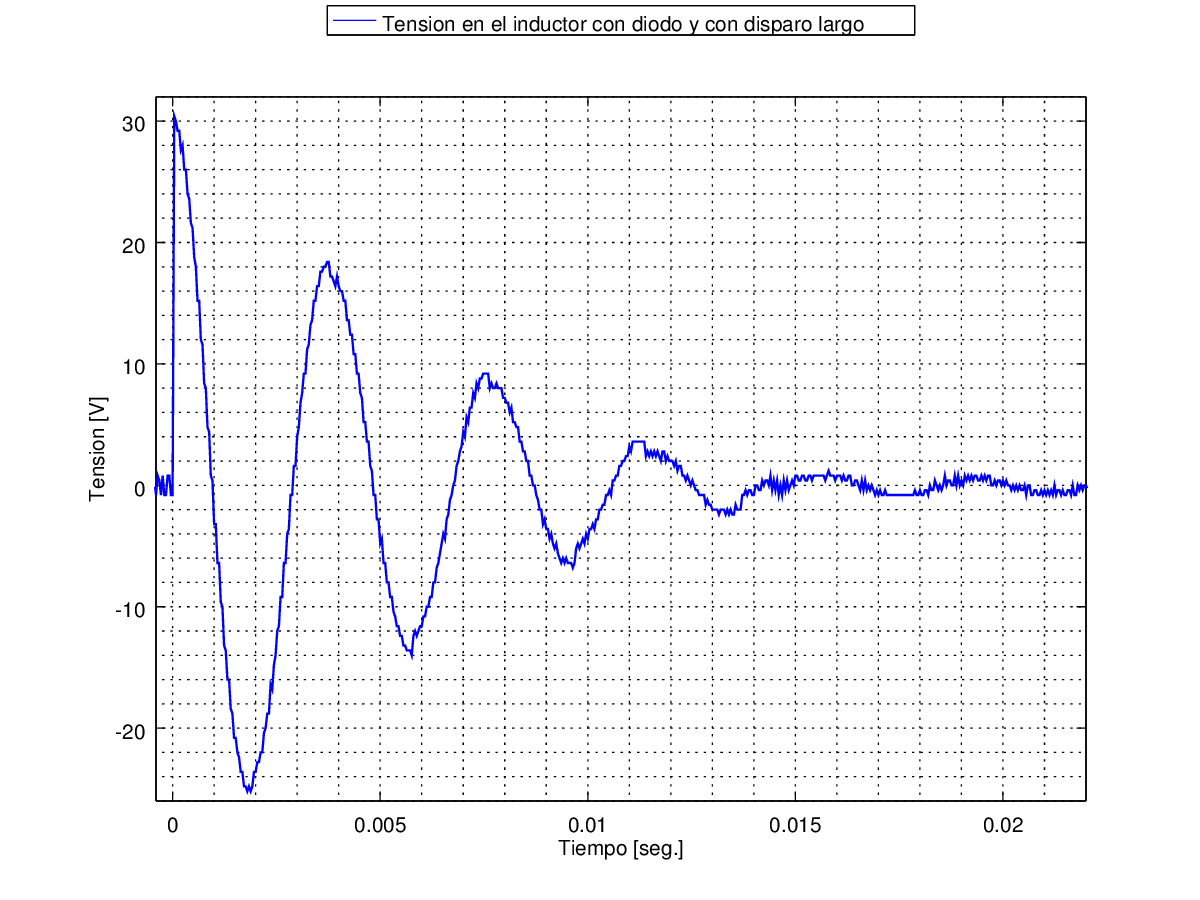
\includegraphics[scale=0.65]{./Octave/tiristores/V_L_con_diodo_disparo_largo.png}
\caption{Tensión en el inductor respecto del terminal negativo de la fuente.}
\label{fig:V_con_diodo_largo}
\end{figure}

\begin{figure}[H]
\centering
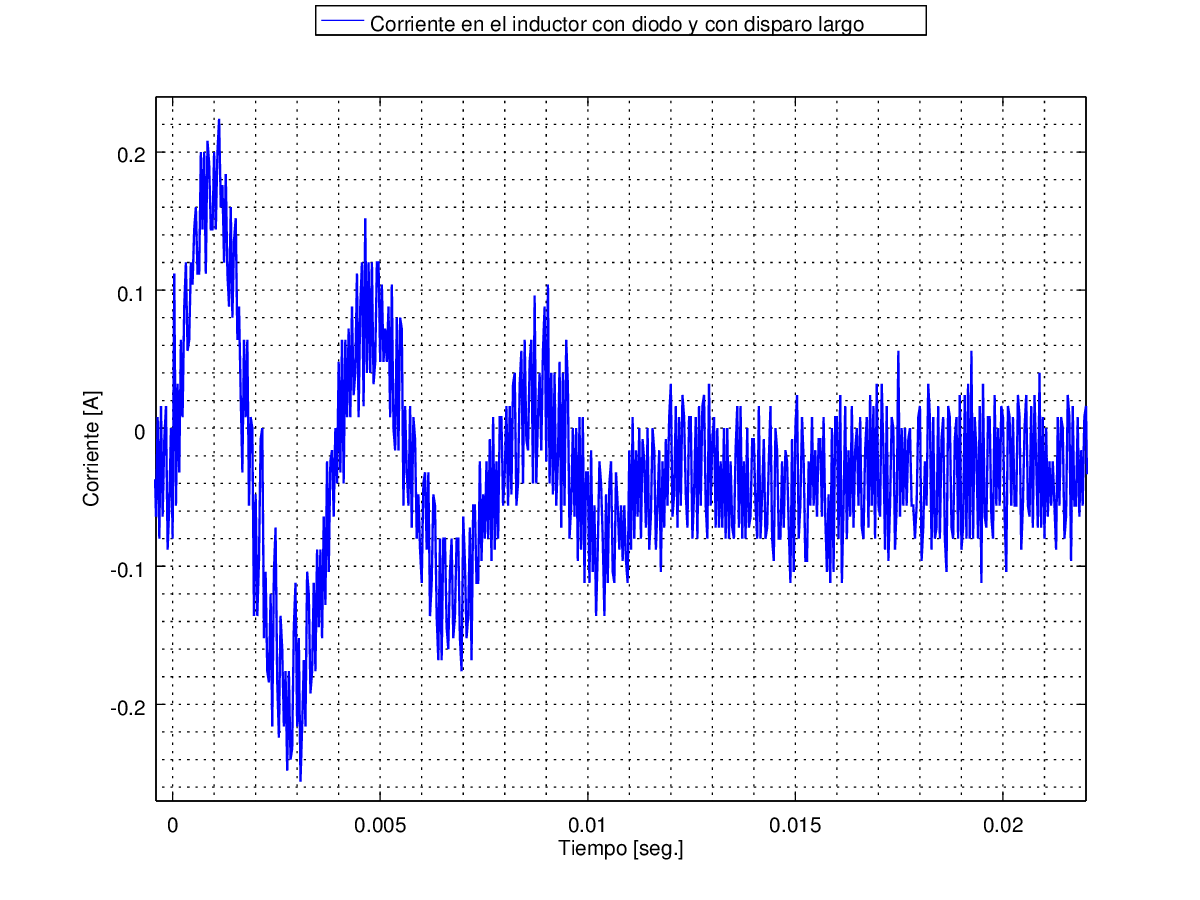
\includegraphics[scale=0.65]{./Octave/tiristores/I_L_con_diodo_disparo_largo.png}
\caption{Corriente en el inductor respecto del terminal negativo de la fuente.}
\label{fig:I_con_diodo_largo}
\end{figure}

\subsection{Análisis de resultados}

\begin{itemize}

\item ¿Porqué se producen distintas formas de onda para cada una de las 
configuraciones medidas?

En la figura \ref{fig:I_sin_diodo_corto} (corriente sin diodo conectado, disparo corto)
se puede  apreciar que la señal termina en $t\simeq 2\,\unit{ms}$, y en la figura 
\ref{fig:I_con_diodo_corto} es en ese punto donde la corriente llega a cero. 
La corriente en el primer caso no puede seguir disminuyendo y volverse 
negativa por la presencia del tiristor, que se comporta como un diodo. 
Una vez que la corriente se extingue, el tiristor no volverá a conducir 
a menos que se le envíe un nuevo pulso al \emph{Gate}.
También se puede apreciar que la corriente no comienza a disminuir hasta que la 
tensión en el tiristor (figura \ref{fig:V_sin_diodo_corto}) se vuelve 
negativa en $t\simeq 0.5\,\unit{ms}$, lo que refleja una propiedad de los tiristores.

En las figuras \ref{fig:V_con_diodo_corto} y \ref{fig:I_con_diodo_corto} 
se puede ver como la señal de tensión en el inductor termina en 
$t\simeq 3.8\,\unit{ms}$. En este punto la corriente que 
circulaba por el diodo no puede volver a circular por el tiristor ya que 
entró en corte cuando se extinguió la corriente que circula por el. 
Esto se debe a que la corriente de base del 
tiristor tiene una duración muy corta, por ende una vez que se 
extinga la corriente del tiristor no volverá a conducir dado que no 
habrá corriente de base que habilite su conducción. 

En cambio en las figuras \ref{fig:V_con_diodo_largo} y \ref{fig:I_con_diodo_largo} se usó 
un disparo largo, y se puede observar que la señal continúa hasta 
extinguirse el transitorio. En este caso la señal usada para habilitar 
la conducción del tiristor tiene una duración mayor que la del transitorio. 
Entonces, la corriente que circulaba por el diodo puede circular 
por el tiristor sin impedimentos porque la señal 
de disparo sigue habilitando la conducción por el tiristor.


\item ¿Porque para cargar el capacitor de $4.7\,\unit{\mu F}$ alcanza con 
realizar un disparo corto?

Una vez disparado el tiristor, éste se mantendrá en conducción hasta 
que la corriente que lo atraviesa caiga por debajo de un valor mínimo 
“holding current”, para este caso $I_H=8\,\unit{mA}$. Una vez activada 
la conducción se trata de un circuito RC, en el cual la conducción se 
deshabilitará cuando la corriente caiga por debajo de $I_H$, pero esto 
no ocurrirá hasta que el capacitor se halla cargado casi en su totalidad. 
Por esto no es necesario que el disparo del tiristor sea largo, alcanza 
con un pulso lo suficientemente largo para habilitar la conducción en 
un primer instante.

\end{itemize}

\section{Conclusiones}

Al utilizar dispositivos de potencia es necesario conocer  los requisitos 
que debe cumplir el dispositivo y dependiendo de si se requiere un dispositivo 
totalmente controlado como los IGBT o semicontrolado como los tiristores. 
Los tiristores al ser semicontrolados sólo dispone de control de la puesta 
en conducción. Los IGBT en cambio variando la tensión del \emph{Gate} pueden 
controlar la corriente que circulan desde el \emph{Colector} hacia el \emph{Emisor}.


Hay que tener en cuenta al utilizar dispositivos de potencia el tiempo de activación.
El tiempo necesario para conmutar el estado de un IGBT dependerá de la 
corriente que circula por su \emph{Gate} hasta cargar su capacitor asociado 
y permitir la circulación de corriente que estará amplificada. En cambio los 
tiristores solo requieren una corriente muy baja para activarse y así permitir 
la circulación de corriente. 


Al manejar corrientes más altas se debe contar con mecanismos de protección, 
como agregar inductores en serie para evitar saltos de corriente. 


Se deben tener en cuenta las temperaturas que alcanzarán los dispositivos, 
ya que pueden llegar a temperaturas elevadas si disipan mucha potencia y 
así dañar el circuito.


En cuanto a los tiristores, el precio a pagar a cambio de un diodo de 
alta potencia es una notable pérdida en el control sobre su funcionamiento. 
También es necesaria la implementación de un circuito adicional para 
generar un pulso que active al tiristor.

\end{document}
